\subsection{Bayesian MCMC Inverse Method}
We implement a Bayesian approach because this method uses past information about the parameter, $h$, to form a prior distribution for analysis and it will sample the posterior probability distribution of ``true" $h$. The recovered distribution of $h$ profiles allows for an intuitive understanding of uncertainty in estimated $h$.

\subsubsection{Bayesian Formulation}

Specifically, we use a Bayesian Markov Chain Monte Carlo (MCMC) method to estimate depth, \textit{h}, given wave number, \textit{k}. %, and wave height, \textit{H}.
This method computes the posterior probability distribution of \textit{h} by combining prior information about \textit{h} with a likelihood function according to Bayes Rule in Equation~\ref{bayes}: 


\begin{equation}\label{bayes}
P(h|%H,
k) \propto \Pi(h)L(h|%H,
k),
\end{equation} 
where $P(h|%H,
k)$ represents the posterior probability function, $\Pi(h)$ is the prior distribution function and $L(h|%H,
k)$ is the likelihood function.

We create a random walk Metropolis algorithm \citep{Metropolis1953} which samples proposed depth profiles and updates the posterior probability distribution of \textit{h} according to the likelihood that the proposed depth profiles describe the true bathymetry. 

To estimate depth, we create a prior distribution function of \textit{h} given 500 realistic approximations of bathymetry derived by the U.S. Army Corps of Engineers.  We assume a normal conjugate prior with mean and standard deviation determined by the distribution of simulated bathymetry as shown in equation~\ref{prior}, this ensures our posterior distribution is normal as well. 

\begin{equation}\label{prior}
\Pi(h) \sim N(0,\sigma_{sim}^2)
\end{equation}
where $\sigma_{sim}^2~=~1.01~m$ is the variance of the simulated \textit{h} profiles. 

Given the sample bathymetry, we evaluate the forward model to compute wave numbers along the 1D profile%and wave heights
. A likelihood function (Equation~\ref{likely}) compares the computed \textit{k} profile to \textit{k} values observed along the 1D profile. 

\begin{equation} \label{likely}
L\left(h|%H,
k\right)=\exp\left(- \frac{\sum\limits_{i=1}^n({k}_{m,i}-k_{d,i})^2}{2\sigma_{d}^2}\right)
\end{equation} 
Modeled and observed \textit{k} are ${k}_{m,i}$ and $k_{d,i}$, respectively, where \textit{i} corresponds to the points along the 1D profile for which we have inferred \textit{k} measurements and $\sigma_{d}^2$ is the variance of \textit{k} values observed along the 1D profile during October 2015. (See section~\ref{datak} for more information about the observations.) 

The likelihood uses the sum of square errors between simulated and observed \textit{k} to quantify the probability that the modeled \textit{k} represents the true \textit{k} profile as observed. Inclusion of the $\sigma_{d}^2$ acknowledges that a perfect match between modeled and observed \textit{k} cannot be expected due to uncertainty in the measurements of \textit{k}.

\subsubsection{Metropolis Algorithm}
The Metropolis algorithm begins with an initial \textit{h} profile sampled from the simulated distribution of bathymetry. This initial estimate of \textit{h} is used to compute an initial prior probability distribution. An initial likelihood probability distribution is computed using observed values of \textit{k}, modeled values of \textit{k} determined by using the sampled \textit{h} as input to the forward model (see Section~\ref{forwardproblem}), and $\sigma_{d}^2$. The prior and likelihood are combined to compute an initial posterior probability distribution of \textit{h}, shown in equation~\ref{post}:

\begin{equation}\label{post}
P(h|%H,
k) = log[\Pi(h)] + log[L(h|%H,
k)]
\end{equation}

The algorithm then uses a markov chain random walk to propose new \textit{h} profiles. Each proposed \textit{h} is evaluated in the forward model to get a proposed \textit{k} profile. The proposed \textit{k} is then compared to observed \textit{k} using the likelihood function and a proposed posterior distribution is computed.

A unique characteristic of the Metropolis algorithm is the way in which proposed posteriors are accepted or rejected by comparison to the previous step's posterior probability. The probabilty of accepting a proposed posterior is 

\begin{equation}\label{accept}
\rho = exp[P(h|%H,
k)_{prop} - P(h|%H,
k)_{current}]
\end{equation}

The formulation in equation \ref{accept} implies that if the proposed posterior probability is higher than the current posterior probability then the proposed posterior probability replaces the current posterior probability and the proposed \textit{h} is accepted as a solution. The algorithm is then incremented and a new proposal is selected and evaluated. 


\subsubsection{Verification}
The Metropolis algorithm used for this project was developed by the authors. To verify the algorithm is working correctly, it was tested on a simple model:

\begin{equation}
y = \alpha x 
\end{equation}
where the algorithm estimates the value of $\alpha$. The true value is known to be $\alpha_{true}=2$. Figure~\ref{verifymcmc} shows that our implementation of the random walk Metropolis algorithm is functioning correctly. We are able to accurately estimate the value of the parameter $\alpha$. 

\begin{figure}[H]
\center
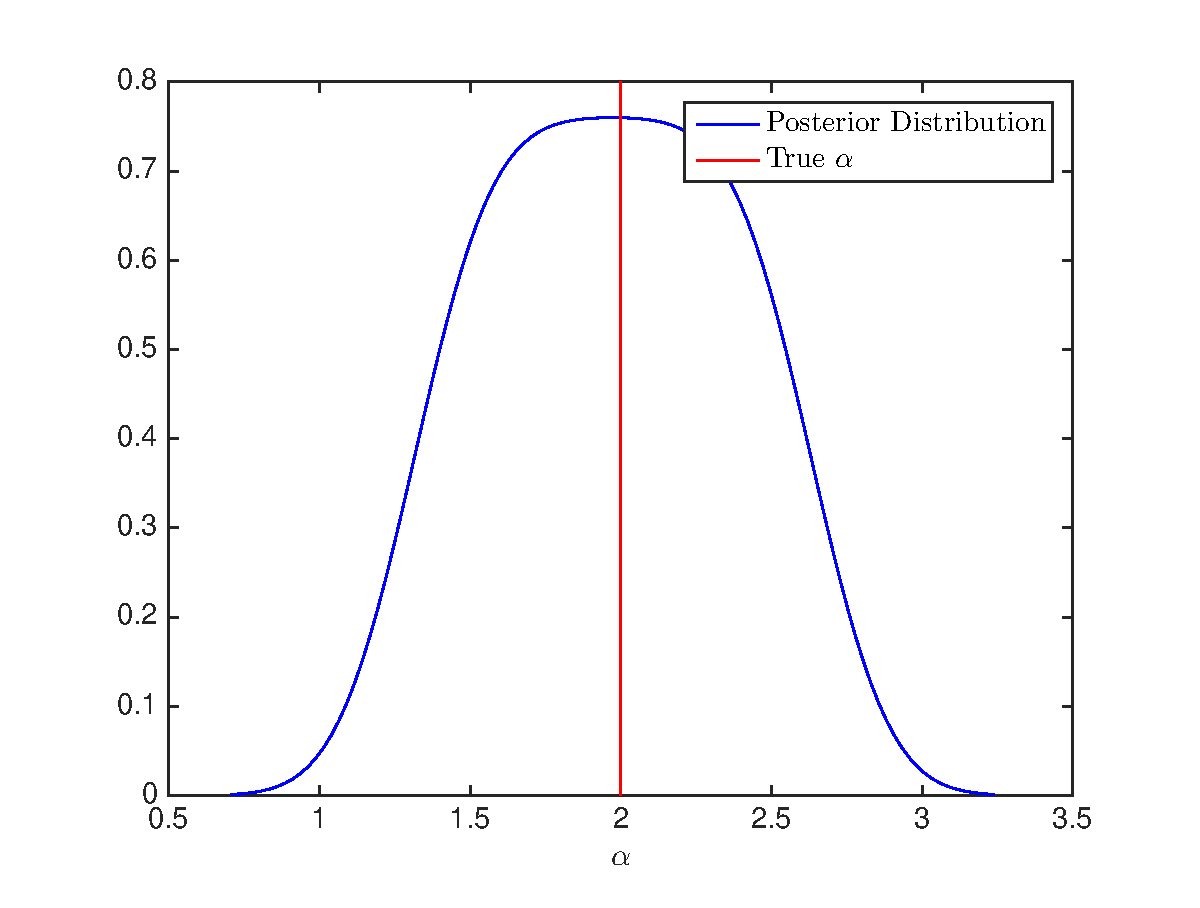
\includegraphics[scale=0.46]{img/MCMC-verification}
\caption{Verification that the Metropolis algorithm has been properly implemented in our code for a simple ODE problem. The red line represents the known value of the parameter $\alpha$. The blue curve is the posterior probabilty distribution sampled by our algorithm. The posterior we compute accurately estimates the true value of $\alpha$.}
\label{verifymcmc}
\end{figure}

For this simple example we add gaussian noise to a sample dataset. The likelihood function is therefore gaussian to account for the gaussian errors:

\begin{equation} \label{likely}
L\left(h|%H,
k\right)=\exp\left(- \frac{\sum({\alpha}_{model}-\alpha_{data})^2}{2\sigma_{d}^2}\right)
\end{equation} 
we use $\sigma_{d}^2$=1 in this case. We use a standard normal distribution for the prior:

\begin{equation}\label{prior_verify}
\Pi(h) \sim N(0,1)
\end{equation}

The proposal step size is 0.5 and the algorithm is iterated 10$^4$ times to arrive at the our example solution, though fewer iterations would have been sufficient. 
















